\dictum[Antisthenes]{I can see a horse, and I can see a man; but
  humanity and horsehood I cannot see.}

\dictum[Plato]{You have the eye which sees a horse and a man; but the
  eye which can see horsehood and humanity you have not.}

\begin{summary}
\item Antisthenis is a framework for building systems for
  \emph{incremental} evaluation of algebraic expressions using
  heuristics to optimize the \emph{order} in which subexpressions are
  evaluated and to calculate some classes of \emph{self referrential}
  computations.
\item \emph{Mealy arrows} are a construct to implement adaptable
  computations that can can produce a value and a new, semantically
  equivalent computation. Each iteration adapts to the previous
  caching values and changing the evaluation plan to be more
  efficient. Antisthenis computations are implemented as network of
  mealy arrows that compose larger adaptive (incremental and partial)
  computations.
\item These Antisthenis processes return concrete values, errors
  (uncomputable values) or partial values (unfinished
  computations). Based on the context of the computation, all kinds of
  values have a lifespan after which computation resets and partial
  values in particular are refined into more concrete kinds of values.
\item Machines are named Antisthenis processes that can be referred to
  by other machines. Antisthenis provides tools for handling some
  classes of self-referential computations.
\item We implement Antisthenis operations to cover requirements of the
  FluiDB physical planner:

  \begin{itemize}
  \item calculate min/sum of natural numbers -- used to compute
    \emph{cost estimations}
  \item boolean functions -- used determine \emph{node materializability}
  \item calculate min/sum of numbers annotated with certainty metrics
    -- used to calculate the estimated cost of materialization of
   n-nodes give nodes that \emph{might} be materialized.
  \end{itemize}
\end{summary}

This chapter goes in depth describing the various parts that compose
Antisthenis, a framework for building incremental computation systems
we developed to assist the FluiDB planner in incrementally and
efficiently computing costs and checking if nodes in the QDAG are
materializable during the evolution of the inventory.

The chapter starts with an introduction about the motivation for
developing Antisthenis as a collection of synchronously communicating
processes performing incremental computation. Next, we look at our
conception of a Mealy arrow that enables the construction of
Antisthenis processes. In the following section we describe the core
of Antisthenis, which is the structure of a single Antisthenis
process. From there we move on to describe some specific operation
implementations that are useful for FluiDB and then describe the
systems that facilitate intercommunication and high level organization
of Antisthenis processes. Finally, we conclude with some caveats and
some future future work that can be done to make Antisthenis easier to
apply to solutions other than FluiDB.

The name Antisthenis is a reference to the proto-empiricist
and proto-nominalist philosophy expressed by Socrates'
pupil Antistenes. Antisthenes promoted particular objects as
preceding universal concepts, encapsulated in his famous
declaration that one can only interact with a horse but not
with the abstract concept of ``horseness''. Antisthenis-the-framework can
compute correct values taking advantage of properties
that are highly specific to the particular computation, potentially
even making use of unfinished intermediate computations.
All that matters to Antisthenis is the computation at hand.

\section{Introduction}
\label{sec:antisthenis_intro}

The order in which subexpressions of an algebraic expression are
evaluated can be important not only for the performance of the
expression evaluation but, in the context of infinite expressions, for
the very termination of the evaluation itself.

Expressions are typically modelled as abstract syntax trees or
computation graphs (DAGs), and evaluation is commonly modelled as a
reduction of that tree or DAG. Depending on the evaluation strategy
each operand is either fully or partially evaluated. Typically, the
strategy for evaluating a subexpression operand , however, is
oblivious to the parent expression and a partially evaluated
subexpression (thunk) is opaque from the perspective of the parent
expression. Breaking this assumption provides some opportunities for
incremental computation and efficient evaluation in the presence of
non-total arguments.

We built \emph{Antisthenis} around this principle to achieve three
important goals:

\begin{itemize}
\item To \emph{incrementally evaluate} an expression, i.e. to only
  re-evaluate the parts of it that depend on parameters that were
  updated with respect to the last time the expression was evaluated.
\item Take advantage of absorbing elements and other operator-specific
  strategies for \emph{early stopping} the evaluation.
\item Often sub-expressions are not total, i.e. they may not be
  computable. A common reason for that is the expression being
  self-referential. These errors may be detrimental to the evaluation
  the top level expression, but often, as we will see, they are not.
\end{itemize}

Incremental computation is a tool for \emph{efficiently} evaluating
expressions of variables that change over time. The area has received
some attention recently
\cite{bhatotiaIncoopMapReduceIncremental2011,hammerAdaptonComposableDemanddriven2014a}. An
incremental evaluator will typically accept a directed acyclic graph
(DAG) of interdependent computations like the following one

\begin{align*}
A &= a + B + C + D  \\
B &= C \times b \\
C & = D + c \\
D &= 0
\end{align*}

Which can be represented as a dag in figure
\ref{fig:example_antisthenis_dag}.

\begin{figure}[H]
\centering
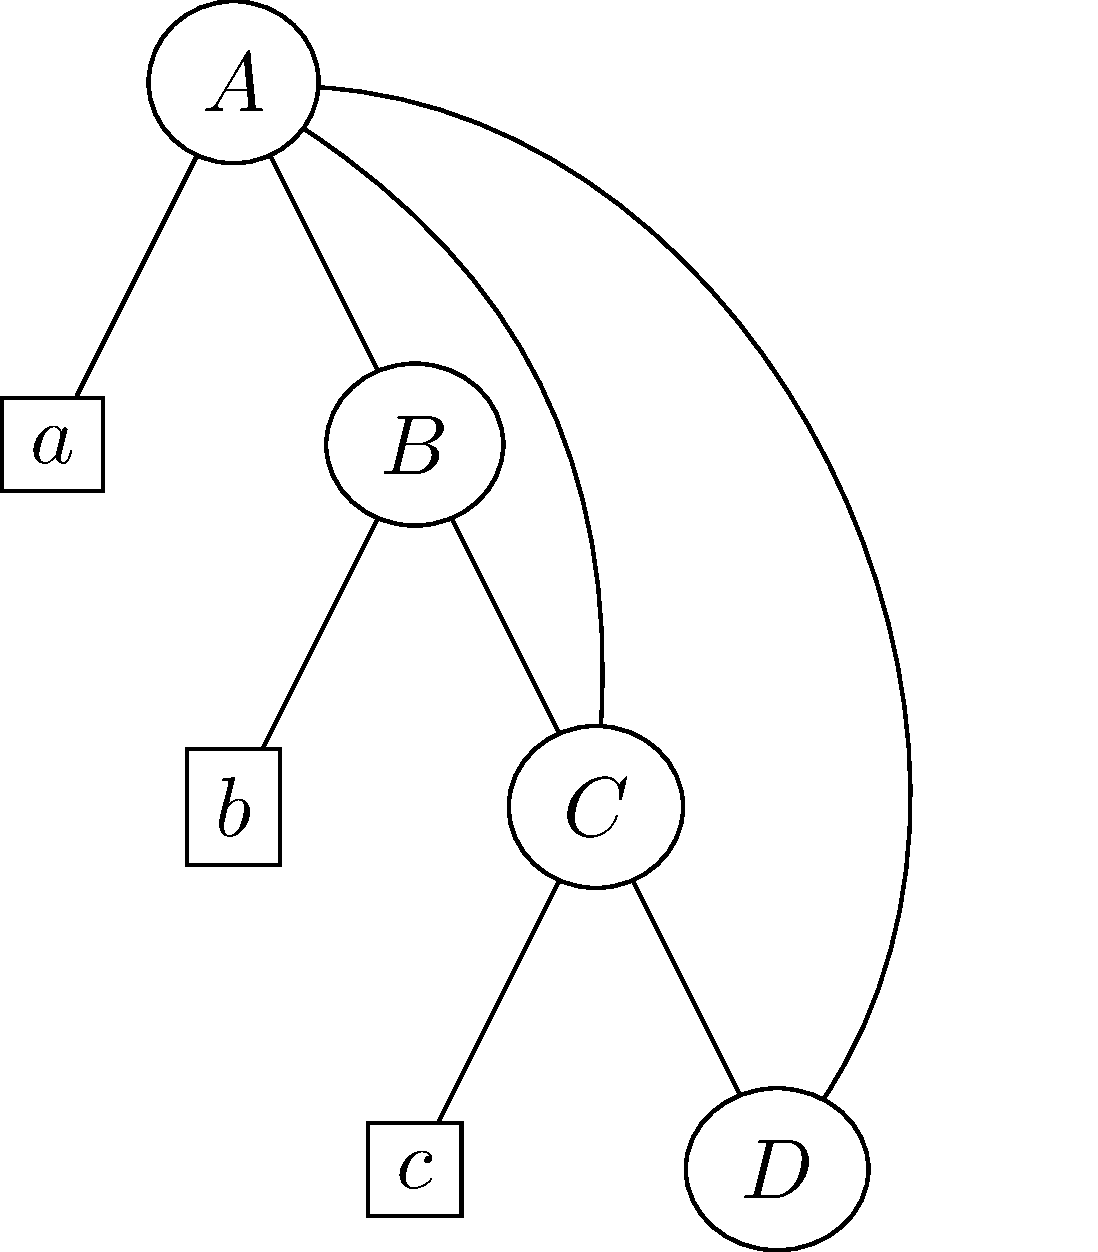
\includegraphics[width=.5\textwidth]{./imgs/example_antisthenis_dag.pdf}
\caption{\label{fig:example_antisthenis_dag}A computation
  DAG. Circular nodes represent operations adn square nodes represent
  parameters that are subject to change.}
\end{figure}

Where \(A\), \(B\), \(C\), and \(D\) are expression nodes in the DAG
and \(a\), \(b\), and \(c\) are parameters that change over time. A
non-incremental evaluation system would evaluate all four nodes every
time a value were requested, regardless of whether and which
parameters have changed. Incremental evalutaion systems keep track of
which variables change and only re-evaluates the nodes of the DAG that
have been updated. In our example, if only the parameter \(b\) has been
updated since the last time \(A\) was evaluated, an evalutation of
\(A\) would require only \(A\) and \(B\) to be re-evaluated.

Incremental evaluation systems employ a wide range of tricks from
simply memoizing the functions
\cite{pughIncrementalComputationFunction1989} to more complex
strategies like Adapton
\cite{hammerAdaptonComposableDemanddriven2014a} where changes in
parameters are propagated in the form of ``dirtying'' DAG nodes and
more explicitly breaking the computation into reusable parts.

To our knowledge, none of the existing approaches to incremental
computation take into account the presence of either absorbing
elements or non-compuatable subtrees (i.e., recursive values) in their
scheduling the evaluation order. Scheduling is either done naively or
left up to the user. However, it is a hard requirement of the FluiDB
query planner for the incremental computing framework to automatically
exploit the properties of the computation at hand in order to
incrementally compute node materializability and query costs in the
presence of different materialized query sets. Furthermore, in all the
approaches we are aware of, the network of sub-expressions was assumed
to be well-behaved, in that all nodes can return a valid value and
there are no cyclical references.

The main principle behind the architecture of Antisthenis is to
manipulate the order in which subexpressions are evaluated in order
to exploit properties of the parent operator and avoid fully
evaluating each of the subterms. For example, when estimating the cost
of a database query, we take it to be the minimum cost of each of
the possible logical plans. It is unlikely that one would need to come
up with a full estimation of each plan, especially the more expensive
ones, before realising the lowest cost. Instead, we would like to
accumulate a lower bound for the cost of each plan.

Another prime example of an opportunity pruning the expression tree is
the exploitation of absorbing elements. In the general case, in a
non-lazy evaluation strategy, to compute the value of a function
\(f(A,B,C)\) where \(A\), \(B\) and \(C\) are expressions, we would
need to fully evaluate \emph{all} three arguments first. Since the
absorbing element of multiplication in the reals is 0, for
\(f(a,b,c) := a \times b \times c\), a result of 0 for the first
argument \(A\) would render the evaluation of the rest of the
arguments redundant.

As alluded to, a lazy evaluation strategy paired with a ``Sufficiently
Advanced Compiler'', can take steps towards mitigating this problem,
but it can only go so far. Consider the following example:

\begin{align*}
A &= B \times C \times D \\
B &= \sum_i{i} \\
C &= 10 - 10 \\
D &= \sum_i{i}
\end{align*}

Here, when evaluating \(A\), a traditional evaluation system would
look at the first argument first, namely \(B\). \(B\) is very
expensive to evaluate and very soon a human would figure out that it
will never evaluate to zero. \(C\), however, does evaluate to zero,
and once that is evaluated, the evaluation of \(A\) is
complete\footnote{Barring domains where infinity needs to be
  considered in any way.}. In a complex set of automatically generated
such expressions it is important that the evaluator does not keep
trying to evaluate a complex expression when evaluating another
simpler one could yield an absorbing value.

Early stopping a computation is useful not only to avoid extra
work. As we mentioned, many incremental computation systems assume
that all sub-computations terminate successfully. Due to reversible
operators, and therefore the QDAG being inherently undirected, the
computations we are interested in will invariably be self
referential. Therefore, we need to take seriously the case where a
sub-expression will fail to terminate. In this case, the parent
expression needs to exhaust all possibilities that could lead to a
value.

\begin{align*}
A &= min(B, C, D) \\
B &= b_1 + b_2 \cdot D \\
C &= c_1 + c_2 \cdot A \\
D &= d_1 + d_2 \cdot B \\
b_1 &= b_2 = d_1 = d_2 = 1 \\
c_1 &= 3 \\
c_2 &= 0
\end{align*}

Here \(B\) and \(D\) are clearly not computable but in the context
where these values represent the cost of evaluations for nodes \(A\)
should evaluate to 3 and \(A\) should evaluate to \(C =
3\). Furthermore, \(A\) should depend \emph{all} parameters for the
validity of its value while \(C\) should depend only on \(c_1\) and
\(c_2\).


\section{Background}

In this section we describe some concepts used to construct the
Antisthenis processese. Here we assume some familiarity with the
common building blocks of effectful computation in Haskell: functors,
applicatives, and monads. They are described in some detail in
appendix \ref{chapter:appendix2}.

\subsection{Arrows and profunctors}

The basic element of computation in the purely functional world is
usually related to the troika of \emph{functors}, \emph{applicatives},
and \emph{monads} \cite{yorgeyTypeclassopedia2009}, in the interfaces
of which we find some recurring substructures that relate their
modification.

\begin{itemize}
\item \texttt{a -> b} the normal pure function type. We take this for granted as
it is provided and managed by the language, in our case Haskell.
\item \texttt{f a -> f b} A functor morphism. The standard functor stack we saw
so far focused on producing such morphisms from simpler arrows.
\item \texttt{f (a -> b)} is known as the Cayley morphism
\item \texttt{a -> f b} which for an \texttt{f} being a monad is the now familiar
Kleisli arrow.
\end{itemize}

We would like to generalize this notion to an parametric object that
we will denote as \hask{~>} (occasionally denoted as \hask{p} ). We
follow the arrow definition from Hughes
\cite{hughesProgrammingArrows2005} which dictates that an arrow must
be a \textbf{category} (i.e. arrows must compose in a commuting way
and there must be an identity arrow) and must also satisfy the
following:

\begin{itemize}
\item It must commute with tuple (i.e., must implement \hask{first} and
  \hask{second}).
\item The Hask category must be embeddable in the category defined by the
arrows (i.e. via the \hask{arr} function)
\end{itemize}

In more concrete terms, we depend on the Haskell typeclasses presented
in listing \ref{lst:arrow_def}. An \hask{Arrow} can act on the first
or second element of a tuple, and an \hask{ArrowChoice} can act on the
the left or the right case of an \hask{Either}.

A related concept to arrows is the profunctor. Profunctors are not
necessarily directly composable like arrows nor do they commute with
tuple or \hask{either}. They only provide \hask{dimap}. \hask{dimap}
is of course implementable in terms of arrow combinators but opting
for dimap can produce much more efficient code.


\begin{code}
\begin{haskellcode}
class Category p where
  id :: p a a -- Maps a value to itself with no effects
  (.) :: p b c -> p a b -> p a c -- composition

class Category c => Arrow p where
  arr :: (a -> b) -> p a b -- arrows do at least what functions can do.
  (>>>) :: p a b -> p b c -> p a c -- also composition
  first :: p a b -> p (a,c) (b,c)
  second :: p a b -> p (c,a) (c,b)
  (***) :: p b c -> p b' c' -> p (b,b') (c,c')
  (&&&) :: p b c -> p b c' -> p b (c,c')

class Arrow p => ArrowChoice p where
  left :: p a b -> p (Either a c) (Either b c)
  right :: p a b -> p (Either c a) (Either c b)
  (+++) :: p a b -> p b' c' -> p (Either a b') (Either b c')
  (|||) :: p a c -> p b c -> p (Either a b) c

class Profunctor p where
  dimap :: (a' -> a) -> (b -> b') -> p a b -> p a' b'
\end{haskellcode}
  \caption{\label{lst:arrow_def}Haskell typeclasses related to the
    notion of \hask{Arrow}.}
\end{code}


All implementations of the interfaces in listing \ref{lst:arrow_def}
are expected to conform to some laws which formalize the intuitions
described about the meaning of arrows. We describe the laws required
for each typeclass to be valid in listings \ref{lst:arrow_laws}

\begin{code}
\begin{minted}{text}
-- | Laws that need to hold for any valid category implementation.
-- Right identity
f . id = f
-- Left identity
id . f = f
-- Associativity
f . (g . h) = (f . g) . h


-- | Laws that need to hold for any valid arrow implementation.
arr id = id
arr (f >>> g) = arr f >>> arr g
first (arr f) = arr (first f)
first (f >>> g) = first f >>> first g
first f >>> arr fst = arr fst >>> f
first f >>> arr (id *** g) = arr (id *** g) >>> first f
first (first f) >>> arr assoc = arr assoc >>> first f

where

assoc ((a,b),c) = (a,(b,c))

-- | Laws that need to hold for any valid arrow choice implementation.
left (arr f) = arr (left f)
left (f >>> g) = left f >>> left g
f >>> arr Left = arr Left >>> left f
left f >>> arr (id +++ g) = arr (id +++ g) >>> left f
left (left f) >>> arr assocsum = arr assocsum >>> left f

where

assocsum (Left (Left x)) = Left x
assocsum (Left (Right y)) = Right (Left y)
assocsum (Right z) = Right (Right z)

-- | Laws that need to hold for any valid profunctor implementation.
dimap id id ≡ id
dimap (f . g) (h . i) ≡ dimap g h . dimap f i
\end{minted}
  \caption{\label{lst:arrow_laws}Laws for the typcalsses related to
    arrows.}
\end{code}

\subsubsection{Examples}

The definition and highlighting of important properties of arrows that
we have done so far is probably not extremely helpful to understand
how computation is defined in such terms. To make the concepts of
arrows and profunctors more tangible, consider the following examples:

\paragraph{The Kleisli arrow}

The \hask{Kleisli} arrow \cite{dawsonCompoundMonadsKleisli2007} as we
mentioned earlier, is equivalent to the arrow \hask{Monad m => a -> m
  b}. In Haskell it is defined as:

\begin{haskellcode}
newtype Kleisli m a b = Kleisli (a -> m b)
\end{haskellcode}

So the arrow \hask{Kleisli (State s) a b} is an arrow that when
mapping values from \hask{a} to \hask{b} also operates on a state
value of type \hask{s}. Composing two Kleisli arrows is equivalent to
binding two \hask{a -> m b} objects using \hask{>=>}. The identity of
the Kleisli category is equivalent to the monadic \hask{return}.

\paragraph{The state arrow}

We already saw the \hask{State} monad in the previous section. If we expand
the \hask{Kleisli (State s) a b} arrow:

\begin{haskellcode}
Kleisli (State s) a b
  ~= a -> State s b
  ~= a -> (s -> (b,s))
  ~= (a,s) -> (b,s)
\end{haskellcode}

The final way of putting it skips a few intermediate steps, we define
a \hask{StateArrow} then as

\begin{haskellcode}
newtype StateArrow s a b = StateArrow ((s,a) -> (s,b))
\end{haskellcode}

Which is equivalent to the Kleisli arrow we created before: an arrow
that when mapping values from \hask{a} to \hask{b} also operates on a state
value of type \hask{s}.

The \hask{StateArrow} is not unique in its equivalence to a Kleisli
arrow. This is a property that a couple of useful arrows have and that
we will be exploiting in the following sections. Below is the
interface we provide to describe the Kleislifieable arrow (named
\hask{ArrowFunctor} below) and a few examples

\begin{haskellcode}

-- | Some arrows correspond to Kleisli arrows. We should be requiring
-- a monad functor but
class Functor (ArrFunctor c) => ArrowFunctor c where
  type ArrFunctor c :: * -> *

  toKleisli :: c a b -> a -> ArrFunctor c b
  fromKleisli :: (a -> ArrFunctor c b) -> c a b

-- | A kleisli arrow is trivially a kleisli arrow
instance Functor m => ArrowFunctor (Kleisli m) where
  type ArrFunctor (Kleisli m) = m
  toKleisli (Kleisli c) = c
  fromKleisli = Kleisli


-- | A state arrow is a state arrow with a bit of rearrangement.
instance ArrowFunctor c => ArrowFunctor (StateArrow s c) where
  type ArrFunctor (StateArrow s c) =
    (StateT s (ArrFunctor c))
  toKleisli (StateArrow c) a = StateT $ \s -> swap <$> toKleisli c (s,a)
  fromKleisli f = StateArrow $ fromKleisli $ \(s,a) -> swap
    <$> runStateT (f a) s

-- | A writer arrow is also a kleisli arrow on top of a writer monad
-- with a bit of rearrangement.
instance ArrowFunctor c => ArrowFunctor (WriterArrow w c) where
  type ArrFunctor (WriterArrow w c) =
    WriterT w (ArrFunctor c)
  toKleisli (WriterArrow c) = WriterT . fmap swap . toKleisli c
  fromKleisli c = WriterArrow $ fromKleisli $ fmap (fmap swap . runWriterT) c
\end{haskellcode}

\subsection{Mealy arrows:  processes that remember}
\label{sec:mealy_arrows}

The concept that we will dub a \emph{mealy arrow} or \emph{mealy
  process}, is kin to many different ideas: transducer, automaton, and
a coroutine to name a few. A mealy arrow (listing \ref{lst:mealy_def})
is a function that along with the result gives a new version of
itself. Like an \emph{automaton} after every iteration it moves to a
new state ready to continue the process. Like a \emph{transducer}
every element of a stream consumed changes a hidden state to be taken
into account when consuming the next one. Like a \emph{coroutine} it
can be conceptualized as a process that can yield computation to be
resumed by the caller.

\begin{code}
\begin{haskellcode}
newtype MealyArrow a b =
  MealyArrow (a -> (MealyArrow a b,b))
\end{haskellcode}
  \caption{\label{lst:mealy_def}Haskell definition of a mealy arrow.}
\end{code}

The mealy arrow is at the heart of Antisthenis as it represents the
basic building block of computation. We call the arrow returned by a
Mealy arrow along with the value an \emph{iteration}. Assuming that a
mealy arrow represents an incremental computation, every iteration is
produced in such a way as to exploit information about the structure
of the problem based on the previous computation.

For example, a mealy arrow calculating a multiplication of several
sub-arrows may want to try the ones that evaluated to zero in the
previous iteration to exploit possible domain knowledge that
nodes that are zero are likely to remain zero in future iterations.

\subsubsection{Mealy arrow transformer}

Like monads \cite{liangMonadTransformersModular1995} , arrows can be
composed to form composite arrow types when they are represented as
\emph{arrow transformers} For brevity we will only talk about mealy
arrow transformers but the concept is generalizable to many different
kinds of arrows \cite{keidelSoundReusableComponents2019a}.

The motivation behind ``transformizing'' the mealy arrow is that arrow
evolution as in the plain mealy arrow we presented must be pure (due
to it being facilitated by \hask{->}). As we will see in detail when
describing the internals of Antisthenis, as subrocesses evolve they
need to interact with external data structures, may throw
irrecoverable errors, need to run monadic computations from external
libraries etc. None of that can be done based on a pure Haskell
function. For that reason, we change the mealy arrow definition
slightly (listing \ref{lst:mealy_trans_def})

\begin{code}
\begin{haskellcode}
newtype MealyArrow c a b =
  MealyArrow (c a (MealyArrow a b,b))
\end{haskellcode}
  \caption{\label{lst:mealy_trans_def}A MealyArrow can take on the
    properties of other arrows by swapping out the function \hask{->}
    type for a parametric one.}
\end{code}

Here the mealy arrow is parameterized by an arbitrary arrow \hask{c}
which may be a Kleisli arrow or any other arrow which will define what
side effects are supported during the evolution of the process.

\subsubsection{Building mealy arrows}

While arrows are powerful and general, they can be slightly awkward to
work with even with the Haskell \hask{proc} syntactic sugar
\cite{bibtex}. Transferring state between mealy iterations via their
closures even more so. Capitalizing on the parallels between an arrow
and a coroutine, and taking advantage of the rich Haskell ecosystem
around monads we define a monad \hask{MB a b m} (standing for \emph{Mealy Builder})
to help us build mealy
arrows more easily. The interface to that monad is presented in
listing \ref{lst:mb_interface}. The \hask{MB a b m x} typed value, as we will
see, can run a computation in \hask{m} and return either a value of type
\hask{x} or a new \hask{MB a b m x}. Thereby, since \hask{Void} is an
uninhabited type, \hask{MB a b m Void} runs a computation in \hask{m}
that \emph{must always} return a new \hask{MB a b m Void}. Just like the
mealy process, only \hask{MB a b m Void} does not expect an argument at
each iteration..

\begin{code}
\begin{haskellcode}
yieldMB :: Monad m => b -> MB a b m a
mkMealy :: (ArrowFunctor c,Monad (ArrFunctor c))
        => (a -> MB a b (ArrFunctor c) Void)
        -> MealyArrow c a b
\end{haskellcode}
  \caption{\label{lst:mb_interface}.The \hask{MB a b m} monad can be
    used as a convenience to implement mealy arrows using a
    conroutine-like interface.}
\end{code}

The important part is that we want to do something before each
iteration, something after, and we want to feed some state to the next
iteration like presented in listing \ref{lst:mb_example}, where it is
how how we can transfer variables between iterations via the closure
of the \hask{do}-block.

\begin{code}
\begin{haskellcode}
foo :: ArrowFunctor c => MealyArrow c a b
foo = mkMealy go where
  go :: a -> MB a b m Void
  go a = do
    b <- mkResult a
    -- Now we got a result we return it to the user and expect the
    -- argument for the next iteration of the mealy arrow
    a' <- yieldMB b
    -- Now both the next argument (a') and the previous result (b) are
    -- in scope. We can use them both. Whatever we do we must
    -- can't simply end the computation. The mealy arrow must
    -- go on.
    go a'
\end{haskellcode}
  \caption{\label{lst:mb_example}An example of the usage of the MB
    functor to generate mealy arrows.}
\end{code}

This involves \hask{toKleisly} in reference to the ``Kleislifiable''
arrows we saw in the previous section and lifting to \hask{MB a b m}
arrow which is precisely defined in \ref{lst:mb_def}. The basis here
is the functor \hask{MealyF a b} which structurally looks like a
non-recursive version of a mealy arrow we saw earlier. That is if
\hask{x} is replaced with \hask{MealyF a b _} we get a mealy arrow
with an extra value. Unfortunately, there is no direct way to make a
law abiding monad out of the \hask{MealyF} type but there is a trivial
functor for it, which allows us to use the free monad
\cite{voigtlanderAsymptoticImprovementComputations2008} to get the
monad we want. Note how the Mealy arrow is \emph{not} kleislifiable
itself. The \hask{MB a b m} monad can't produce any mealy arrow. We
can produce only arrows that are from \hask{a} to \hask{b} from
\hask{MB a b m Void}.

\begin{code}
\begin{haskellcode}
-- | Constructing monadic xmealy arrows
newtype MealyF a b x = MealyF (a -> x,b)
type MB a b = Free (MealyF a b)
\end{haskellcode}
  \caption{\label{lst:mb_def}Definition of the MB monad transformer.}
\end{code}


\subsection{Zippers}

Now that we have a fairly coherent view of computations, we need one
more piece of background to start putting together Antisthenis: the
zipper data structure. A zipper \cite{huetZipper1997} is an auxiliary
data structure that is similar to (but not exactly the same as) a
cursor.

For our purposes a zipper is a data structure that represents an
alternative configuration of a container such that it focuses on a
specific location in that container, allowing an interface for reading
and modifying the element at that location. A zipper should also be
able to shift focus to adjacent elements.

Zippers can be very complex data structures with interesting
categorical properties arising from the fact that they can implement a
command interface \cite{uustaluComonadicFunctionalAttribute2005} but
for our purposes we only need a rudimentary understanding of it.

As an example, consider the structure \hask{ListZipper}:

\begin{haskellcode}
data ListZipper =
  ListZipper
  { lzLeft :: [a]
   ,lzCur :: a
   ,lzRight :: [a]
  }
\end{haskellcode}

A list zipper breaks the list in three parts: a left part \hask{lzLeft}, a
focused element \hask{lzCur} and a right part \hask{lzRight}.

\begin{haskellcode}
-- Make a zipper from a non-empty list
mkZipper :: [a] -> Maybe (ListZipper a)
-- get a list from the zipper
getList :: ListZipper a -> [a]
-- Focus on an element on the left if there is one
moveLeft :: ListZipper a -> Maybe (ListZipper a)
-- Focus on an element on the right if there is one
moveRight :: ListZipper a -> Maybe (ListZipper a)
-- Modify the current element
modCur :: (a -> a) -> ListZipper a
-- Read the element in focus.
getCur :: ListZipper a -> a
\end{haskellcode}

These are fairly self-explanatory, a zipper can shift focus from the
element in question to the neighboring elements.

\section{Antisthenis core}

The parts that comprise Antisthenis are roughly split in two
categories.

\begin{itemize}
\item The \emph{core components} that are related to building the
  Antisthenis processes, the cells of computation, and the interfaces
  that need to be implemented to specialize them to specific
  operations.
\item and the \emph{external components} that generally relate cells
  to each other and the systems that specialize proecesses to
  implement specific operators.
\end{itemize}

While in this section we focus on the core components and we will
frequently allude to external components, which we will see in detail
in sections \ref{sec:antisthenis_ops} on operators and
\ref{sec:antisthenis_machines} on named processes.

\subsection{Processes}
\label{sec:antisthenis_processes}

An Antisthenis process is a node in the evaluation graph and it is
built using the concepts described so far in order to implement the
following properties:

\begin{itemize}
\item \emph{Parameterize} the computation by a cascaded configuration
  (as we will see \hask{Conf w})
\item \emph{Adapt} the computation between runs using Mealy arrows.
\item Return metadata about the result \emph{deliniating its validity}
  (as we will see \hask{CoEpoch w})
\item Disambiguate betweeen an \emph{uncomputable}, a \emph{partial},
  and a \emph{concrete} result (as we will see \hask{BndR w})
\end{itemize}

As we described in section \ref{sec:mealy_arrows} mealy arrows define
the basis of an Antisthenis process. Indeed, our definition of an
Antisthenis incremental cell is a composition of \hask{MealyArrow},
\hask{WriterArrow} and \hask{Kleisli} presented in
\ref{lst:arrproc_def}

\begin{code}
\begin{haskellcode}
type ArrProc w m =
  MealyArrow (WriterArrow (ZCoEpoch w) (Kleisli m))
  (Conf w) (BndR w)
\end{haskellcode}
\caption{\label{lst:arrproc_def}The type of an Antisthenis process is a Mealy arrow paired
  with a kleisli arrow.}
\end{code}

The \hask{w} parameter is simply a token related to the operation that
the cell is evaluating that we use helps us parameterize the types
involved in a process by leveraging the type family feature of
Haskell's type system \cite{AssociatedTypeSynonyms}. We call it a
\hask{ZipperParams} tag because, as we will be seeing throughout the
chapter, it mainly parameterizes the evolution of the internal state
of the Antisthenis process, the \hask{Zipper}.

We will describe every type involved in the \hask{ArrProc} type
separately, but to do that we first provide a general intuition of
what these types mean. The basis is a mealy arrow that emits a
monoidal value \hask{ZCoEpoch w} via \hask{WriterArrow} that expresses
metadata, along with the result of the computation (\hask{BndR w}).
It is a datastructure that summarizes the provenance of the value
returned described in detail in section \ref{sec:caps_and_bounds} on
Antisthenis caps and bounds. It is used to determine when the value is
no longer valid, for example, due to changed parameters.

The \hask{MealyArrow} and \hask{WriterArrow} combined transform an
arbitrary Kleisli arrow which is used to embed the computation of
Antisthenis processes into parent monadic computations, which in the
case of FluiDB is the \hask{PlanT t n m} monad as we saw in section
\ref{sec:planner}. In the FluiDB case, that would be the monad
computation associated with planning. This way we give the
Antisthenis processes the means to lookup values, throw errors, or
generally have the effects of any computation we require.

The output side of the \hask{ArrProc} is a \hask{BndR w} type, the
returned value, which is parametric to the operation but has some
common structure (listing \ref{lst:bnd_def}). This indicates that every
Antisthenis process has three options for the value they can return
all of which are parameterized on a per-operation basis (ie
\hask{ZErr}, \hask{ZBnd} and \hask{ZRes} are type families):

\begin{itemize}
\item An error indicates that the value is not computable.
\item A final and precise result.
\item A partial result, a convex bound indicating that calling the
  iteration of the arrow will get us closer to ax` final result. We will
  have a chance to see the bounds in detail in the section
  \ref{sec:caps_and_bounds} on caps and bounds.
\end{itemize}


\begin{code}
\begin{haskellcode}
data BndR w
  = BndErr (ZErr w)
  | BndRes (ZRes w)
  | BndBnd (ZBnd w)
\end{haskellcode}
  \caption{\label{lst:bnd_def}The definition of the return value of an
    Antisthenis process. It may be a final result, an error indicating
    that a final result is non-computable, or a bound for the final
    value.}
\end{code}

Indeed, the iteration of the process has a very different meaning
depending on whether the previous returned value is a bound or an
error/result. In the former case the iteration continues a previous
computation, in the latter there are two options.

\begin{itemize}
\item The previously returned value is still valid and is therefore
  returned,
\item If it is not and the computation is reset.
\end{itemize}

To reflect this fundamental difference between a paused and a finished
computation we will call the former simply an \emph{iteration} and the
latter \emph{coiteration}.

Finally, we turn our attention to \hask{Conf w} which represents the
configuration for running the next step of the computation. Much like
\hask{BndR} the configuration is parameterized w.r.t. \hask{w} but has
a basic structure presented in listing \ref{lst:conf_def}

\begin{code}
\begin{haskellcode}
data Conf w =
  Conf { confCap :: Cap (ZCap w)
        ,confEpoch :: ZEpoch w
       }
\end{haskellcode}
  \caption{\label{lst:conf_def}The type definition of a
    conficuration. It is a tuple containing information that can be
    used to derive whether a value is valid.}
\end{code}

The configuration for running a computation includes an \emph{epoch}
that is used to deprecate computed values that are no longer valid
(discussed in section \ref{sec:epochs_coepochs}) and a \emph{cap} that
is used to decide when a partial result should be returned (discussed
in \ref{sec:caps_and_bounds}). The configuration is passed as input to
each computation and propagated to the children computations. If the
process is iterating (as opposed to co-iterating, i.e., it has not
returned a concrete result or an error), the cap is compared against
the previously yielded bound, if the cap is less than the bound
returned then the process must keep processing until it finds a bound
that exceeds that cap. This way we can control how much work a process
is allowed to do before switching to one that might help Antisthenis
to cut the overall computation short. This way, Antisthenis avoids
falling into computational rabbit holes, where it evaluates a longer
computation when switching to a shorter one would help arrive sooner
to a final result.

The \emph{epoch} represents state external to Antisthenis like
parameter versions. When the epoch indicates that a parameter on which
the process depends has been updated, the process needs to be reset
and start the computation from scratch (see section
\ref{sec:process_resetting} on process resetting).


\subsection{Epochs and coepochs}
\label{sec:epochs_coepochs}

As mentioned in the previous section, the interplay between epochs and
coepochs determines the validity of the value of each Antisthenis
process. When the returned value is no longer valid the process needs
to be reset; in particular, the epoch mainly indicates the ``version''
of the computation parameters. This might represent the full external
state, but the purpose of the epoch is to be used as an increasing
value that can be used by the processes to infer whether their
progress is based on out-of-date assumptions. For example, the epoch
may be a map of a natural number per computation parameter indicating
the number of times that parameter has been updated. Or it might
simply be the actual value of each parameter if it is cheap the
compare against. Each process then can compare the version or value of
each parameter of the epoch to the ones it used to build its internal
state. When a discrepancy is found the process knows its state is out
of date and must reset.

It is clear that not all parameters are relevant to all processes.
Most processes only depend on a subset of parameters, or in
Antisthenis' terms, most processes only ever depend on parts of the
epoch. This reference to a subset of any epoch is reified by the
\emph{coepoch}. The coepoch is the monoidal type parameter of the writer
arrow transformer of \hask{ArrProc}.  In practice this means that due
to the writer semantics, the coepochs of evaluated subproecesses are
concatenated to produce the coepoch of the parent process. A special
case for this are the commutative operations that involve absorbing
elements (\(\land\), \(\lor\), and \(\times\)), where only the coepoch
of the subprocess that yields an absoring element is returned. In
short, the coepoch of a subprocess is included in all parent processes
that are not constant with respect to the value of that subprocess.

In principle, the function that the \hask{ZipperParams} tag needs to
implement to facilitate the epoch/coepoch interplay is a function that
has a type equivalent to listing \ref{lst:comb_epoch_coepoch0}.

\begin{code}
\begin{haskellcode}
combEpochCoepoch0 :: ZEpoch w -> ZCoEpoch w -> Bool
\end{haskellcode}
  \caption{\label{lst:comb_epoch_coepoch0}The type of a naive function
    checking the validity of a value based on epoch and coepoch.}
\end{code}

That will indicate whether the value needs to be pushed down. In
practice we can do slightly better at that by enforcing the following
law on the \hask{combEpochCoepoch0} function:

\begin{align*}
& \text{combEpochCoepoch}_0(e, c_0 \diamond c_1) \Rightarrow \\
& \text{combEpochCoepoch}_0(e,c_0) \land \text{combEpochCoepoch}_0(e,c_1)
\end{align*}

Where \(e \in \mathit{ZEpoch w}\), \(c_0,c_1 \in \mathit{ZCoEpoch w}\)
and \(\diamond\) is the monoidal merging operation on coepochs.

We therefore have the option of filtering the epoch into a smaller
subset of itself that is only relevant to the subprocesses that
contributed to the generation of the coepoch being checked. Thereby
the combination function can optionally return a new epoch, rendering
the type of the function to be something similar to listing
\ref{lst:comb_epoch_coepoch}. It is worth noting that if by this
process we determine that a reset is required, a new coepoch is also
required and therefore there is no way to constrain the epoch to run
the reset process.

\begin{code}
\begin{haskellcode}
combEpochCoepoch :: ZEpoch w -> ZCoEpoch w -> Maybe (ZEpoch w)
\end{haskellcode}
  \caption{\label{lst:comb_epoch_coepoch}The final function for epoch
    and coepoch combination.}
\end{code}

\subsection{Antisthenis caps and bounds}
\label{sec:caps_and_bounds}

In section \ref{sec:epochs_coepochs} regarding epochs and copeochs we
described how Antisthenis deals with the validity of values returned
by a process.  In this section we will focus on how the children
processes avoid falling into avoidable computational rabbit holes
using the interplay of \emph{caps} and \emph{bounds}.  In the example
discussed in the introduction of this chapter
(\ref{sec:antisthenis_intro}), we saw that there are cases where, as
soon as a subprocess can prove that its value is going to exceed a
certain threshold (\emph{cap}) any further work on its part is likely
futile. It then returns a \emph{bound} which is propagated up the
chain of parent processes and handled at the point where the cap was
imposed.  The reader is encouraged to maintain a mental model where
the cap is an threshold and the bound is a lower bound.

We expect that the bound of a function satisfies the
\emph{mototonicity criterion}:

\[
C \dot{<} B[ f(a_0, ...)] \Rightarrow C \dot{<} f_B(B[a_0],...)
\]

Where \(C\) is the cap, \(B[E]\) is the bound of a process expressed
by the expression \(E\) by only taking into account the top level
terms. \(f\) is the function of the operator and \(f_B\) is a function
that combines the bounds of the arguments to come up with a bound for
\(f\). \(C \dot{<} b\) means that the bound \(b\) exceeds the cap
\(C\). In simpler terms, this means that if a bound exceeds the cap,
evaluating the arguments and coming up with tighter bounds will still
exceed the cap.

There may be more requirements of the properties of a cap w.r.t. a
particular operator. For example, the minimum operator requires that
bounds be translatable to caps and that if a bound \(b\) is translated
to a cap \(c\) and \(b' \dot{<} c\) then \(b' < b\). This requirement
is only related to the way the particular operator is implemented and
is not necessarily a requirement for any other operator.


The \hask{ZipperParams} tag \hask{w} needs to provide a way for
comparing caps to bounds. Unlike the case of coepoch and epoch
combination function this one is much more straightforward:

\begin{haskellcode}
exceedsCap :: ZCap w -> ZBnd w -> Bool
\end{haskellcode}

Simply given a cap and a bound, check if the bound exceeds the cap. A
special case of a cap is \hask{ForceResult} for which
\hask{exceedsCap ForceResult _ == False}. As the name suggests
\hask{ForceResult} is used when we want a process to necessarily
return a concrete result or an error, as opposed to a bound.

Now that we have seen how the cap is handled on the input side we
should discuss how the parent process passes a cap to its child
processes. The cap is created in an operator-specific way (i.e., via the
overloading of a function based on the tag \hask{w}). In particular an
operator defines a function that ``localizes'' the entire configuration.

\begin{haskellcode}
data MayReset a = DontReset a | ShouldReset
zLocalizeConf :: ZCoEpoch w -> Conf w -> Zipper w p -> MayReset (Conf w)
\end{haskellcode}

The \hask{zLocalizeConf} function accepts a coepoch, the configuration
that the parent process receives and returns the configuration
passed. The \hask{zLocalizeConf} function also decides whether the
process needs to be reset by calling the \hask{combEpochCoepoch}
function that we discussed in subsection \ref{sec:epochs_coepochs} on
epochs and coepochs.

To make all this more tangible, a process that computes the sum of its
subprocesses might implement \hask{zLocalizeConf} roughly like shown
in listing \ref{lst:localizeconf}. Since the process knows it will be
evaluating the cursor, it subtracts the partial sum so far from the
cap to come up with the cap to pass to the subprocess.


\begin{code}
\begin{haskellcode}
zLocalizeConf coepoch conf z =
  combEpochCoepoch coepoch (confEpoch conf)
  $ conf { confCap = newCap
         }
  where
    -- zRes is the partial result so far
    newCap = case zRes z of
      SumPartErr _ -> error
        $ "The partial sum is an error: this thunk "
        ++ "should never be reacahble beacuse "
        ++ "no subprocesses should be called."
      SumPartInit -> confCap conf -- No subprocesses have been evaluated.
      SumPart partRes -> case confCap conf of
        -- partRes is the total sum so far. We offset the global cap
        -- by the sum so far so that the local cap ensures that the
        -- cursor process, when ran, does not cause the overall
        -- bound to exceed the global cap. This may generate weird
        -- caps like negative values. That is ok as it should be
        -- handled by the evolutionControl function. Note again that
        -- zRes does not include the value under the cursor.
        CapVal cap -> CapVal $ subCap cap partRes
        ForceResult -> ForceResult
\end{haskellcode}

  \caption{\label{lst:localizeconf}A sample implementation of the
    function that transforms the configuration received by a parent
    process into one suitable for the child process. Checks if the
    parent process needs to be reset and uses the partial result to
    constrain the cap. This particular implementation is taken from
    our implementation of the sum operator.}
\end{code}

\subsection{Antisthenis zipper}
\label{sec:zipper}
We saw in the introduction of Antisthenis
(section \ref{sec:antisthenis_intro}) what a zipper is in general. Here we
will specialize the notion for the specific case of the internal state
of the computation. A single process is defined by an operator, the
subprocesses and a partial result for the computation. The process
evolves by evaluating a subprocess at a time. We define a zipper
structure that:

\begin{itemize}
\item Focuses on the particular process to be evaluated next.
\item Arranges a reset process that restarts the evaluation from a
  state that possibly takes into account information about the
  previous evaluation, for example, by starting evaluation from a
  subprocess that previously yielded an absorbing element.
\end{itemize}

With this in mind, we define the zipper data structure keeps track of
the state of the node (see figure \ref{fig:zipper}).

\begin{itemize}
\item A set of \emph{initial} processes that have not been evaluated
  yet or that have yielded deprecated values (see section
  \ref{sec:epochs_coepochs} on epochs and coepochs).
\item A set of \emph{iteration} processes, processes whose latest
  evaluation has yielded a result bound is represented by a data
  structure that associates the iteration processes with initial
  processes bounds returned. Since these processes that have yielded a
  value bound and need to be rerun with a different cap (see section
  \ref{sec:caps_and_bounds}). It should be stressed that this still
  acts like a heap of subprocesses where the internal properties of
  the data structure decide the top element that is to be
  popped. Since we have some information about the final result of
  these processes, namely the bound, the parent process can be smart
  about the order in which they are evaluated. As the particular
  strategy depends on the operation implemented by the parent process,
  the particular data structure used is also dependent on said
  operation. For example, a process implementing a sum between the
  subprocesses stores them in a list as there is no beneficial order
  in which to evaluate the subprocesses, while minimum operation
  benefits from evaluating the processes that have lower bounds first
  (for more details on the minimum operation see section
  \ref{sec:basic_cost_ops}).

\item \emph{Coiteration processes} are processes that have been
  evaluated and yielded a concrete value (error or result), i.e., a
  value that is predicated on the epoch but can not be refined by
  re-evaluating the process with a more permissive cap. Upon reset the
  coiteration stack is ordered in an operator-specific way and moved
  to the init stack.
\item A \emph{cursor} that is the next process to be triggered along
  with a way to reset it and the previous value.
\item A \emph{partial value} to which values can be inserted or
  removed (for example the sum accumulated up to that point) which
  represents the progress of the process so far. As values, concrete
  or partialm are extracted from the subprocesses the partial value is
  updated. The partial value does \emph{not} include the value stored
  in the cursor.
\end{itemize}

\begin{figure}[H]
\begin{tikzdiagram}
  \tikzset{b/.style={circle,draw,minimum size=1cm}};
  \tikzset{m/.style={circle,draw,minimum size=1cm, fill=gray!10}};
  \tikzset{node/.style={rectangle}};
  \tikzstyle{background}=[rectangle, fill=gray!10, inner sep=0.2cm]

  \node[node] (sep) {};


  \newcommand{\mkmat}[4]{
    \matrix (#1) [#2,background,nodes={align=center,minimum height=2em},label=above:#3]{
      \node[node] {#4}; \\
      \node[node] {#4}; \\
      \node[node] {#4}; \\
      \node[node] {#4}; \\
      \node[node] {...}; \\
      \node[node] {}; \\
    };
  }
  \mkmat{its}{above=of sep}{Iterations}{\((b,p_{reset},p_{it})\)}
  \mkmat{init}{left=of its}{Initials}{\(p_{init}\)}
  \mkmat{coit}{right=of its}{Coiterations}{\((p_{coit},r)\)}

  \node[below=of sep,background,label=below:Cursor] (curs) {\((Maybe[b],p_{reset},p_{rg})\)};

  \path[-stealth,bend right=20] (init.south) edge node[midway,fill=white] {cmd init} (curs.west) ;
  \path[-stealth,bend right=20] (its) edge node[midway,fill=white] {cmd it} (curs) ;
  \path[-stealth,bend right=20] (curs) edge node[midway,fill=white,text width=1cm] {Bounded\\result} (its) ;
  \path[-stealth,bend right=20] (curs.east) edge node[midway,fill=white,text width=1cm] {Final\\result} (coit) ;
\end{tikzdiagram}
\caption{\label{fig:zipper}The zipper splits the sub-processes that
  cooperate to compute values for the owning process in four
  categories a) initials that have not yielded a currently valid value
  b) iterations that have not yielded a valid partial value c)
  coiterations that have yielded a full valid value d) the cursor that
  is the next sub-process to be evaluated.  Depending on the
  evaluation strategy of the operator once the cursor process is
  evaluated it is replaced with an init process or an iteration
  process, and depending on the value the cursor process yields it is
  pushed to the iterations or the coiterations of the zipper.}
\end{figure}

During computation, the subprocesses owned by the parent process are
evaluated, and their iterations are then moved from the \emph{initial}
process set to the \emph{coiteration} process nset, possibly with an
intermediate stop in the \emph{iterations} set according to the values
and strategies of the operator implementation which is further
elaborated in section \ref{sec:antisthenis_ops} on Antisthenis
operations. The structure of \emph{iterator set} is highly operator
dependent and primarily geared towards efficiently evaluating the
parent process, but fundamentally it must not compromise on the
correctness of the operator. For example, a process is combining
elements of an Abelian group (commutative, associative, invertible)
and the bound has the same type as the result -- as it is the case
with addition -- the structure of the zipper is fairly
straightforward:

\begin{itemize}
\item The partial result maintains the aggregation of all values and
  bounds encountered.
\item When evaluating the cursor we add the result or returned bound to the group and
  remove the bound of the next cursor if we are popping from the
  iteration set.
\item The bound of the final value at any moment is the partial
  result.
\end{itemize}

At the other end of the spectrum, a process evaluating a magma (a set
with a closed binary operation), where the binary operator has no
properties besides closure, must never push anything to the iterations
set. The set is equivalent to unit (\hask{()}), and the cursor is
forced to yield a concrete result or an error by being run with a
\hask{ForceResult} cap.

To make the concept tangible, below are some examples of what the iterator set is
defined as for different operations (all numerical operations are
assumed to operate on non-negative numbers, in particular query
costs):

\begin{itemize}
\item Addition is the simplest case: the iteration set is an
  always-empty container since we always evaluate the cursor until it
  is sent to the coiteration list. In the context of addition there is
  no heuristic to predict which subprocess is more beneficial to
  evaluate.
\item For multiplication over positives, we evaluate the ones
  that have a zero bound first hoping that they will turn out to
  evaluate to absorbing elements. Therefore, the iteration set is
  represented as two lists: one where the zero-bounded iterations
  are stored and one for the rest.
\item In the case of the minimum operator the iteration set is a heap. In each step we
  evaluate the one with the minimum bound. When the minimum
  bound exceeds the minimum concrete result encountered, the min concrete
  result is the final result.
\end{itemize}

For completeness, we provide the definition of the \hask{Zipper} in
listing \ref{lst:zipper_def}

\begin{code}
\begin{haskellcode}
 data ZipState w a =
  ZipState
  { bgsInits :: [InitProc a]
   ,bgsIts :: ZItAssoc w (InitProc a,ItProc a)
   ,bgsCoits :: [(Either (ZErr w) (ZRes w),CoitProc a)]
  }

data Zipper' w cursf (p :: *) partialRes =
  Zipper
  { zBgState :: ZipState w p
   ,zCursor  :: cursf (Maybe (ZBnd w),InitProc p,p)
   ,zRes     :: partialRes -- The partial result without the cursor.
  }
type Zipper w p = Zipper' w Identity p (ZPartialRes w)
\end{haskellcode}
  \caption{\label{lst:zipper_def}The definition of the zipper.}
\end{code}

Finally, each operator defines the type of the partial result (\hask{ZPartialRes})
maintained in the zipper, as well as functions for putting and replacing values in
it. When the subprocess of the cursor is evaluated the result needs to
be either ``appended'' into the partial result if the new cursor is
drawn from the initials set, or to replace the corresponding bound
value if it is replaced with a value from the iterations set.

\subsection{The Cmds functor}
\label{sec:cmds_functor}

As indicated in section \ref{sec:zipper} on Antisthenis zippers
the process evolution is guided
by shifting the zipper focus to different subprocesses and then
evaluating them.

A process is internally represented as a Mealy arrow (introduced in
section \ref{sec:mealy_arrows}) describing the evolution of a
\hask{ZProc} which is transformed into the Antistehnis process
described in section \ref{sec:antisthenis_processes} by following the
strategy in which the \hask{Zipper} is meant to evolve. An operator is
allowed to follow a strategy defined specifically its
\hask{ZipperParams} tag, but the function for evaluating said strategy
applies to the \hask{ZProc} object. There are two important aspects to
be noted about \hask{ZProc} (listing \ref{lst:zproc_def}).

\begin{itemize}
\item The return value is a zipper full of processes \hask{Zipper w
    (ArrProc w m)}
\item The Kleisli arrow is a free functor of commands \hask{FreeT
    (Cmds w) m}.
\end{itemize}

\begin{code}
\begin{haskellcode}
type ZProc e m =
  MealyArrow
    (WriterArrow (ZCoEpoch w) (Kleisli (FreeT (Cmds w) m)))
    (LConf w)
    (Zipper w (ArrProc w m))
\end{haskellcode}
  \caption{\label{lst:zproc_def}An internal representation of the
    process evolving the internal representation of a process: the
    zipper. Note the use of \hask{FreeT Cmds} in the Kleisli arrow.}
\end{code}


\hask{Cmds}, used in type parameter of the Kleisli arrow in
\hask{ZProc}, is a union type encapsulating different directions to
which the zipper can be evolved. Its definition is provided in listing
\ref{lst:cmds_def}. The point of \hask{Cmds} is to separate the logic
of \emph{how} each possible zipper transition is carried out which is
largely operator agnostic, from the logic of \emph{which} transition
should be carried out which is higly operator dependent.  \hask{ZProc}
is therefore a process that simulataneously encapsulates all possible
evolution paths for the zipper.  The command constructors reflect the
different evolution steps that can be taken at each time:

\begin{itemize}
\item It can always be reset the process
\item It can pop a process from the initial to the cursor to be executed
\item It can pop a process from the iterator set if it is not
  empty. Which one is to be popped is decided by the parameters
\item The may have reached a final value where it can't be evolved
  anymore.
\end{itemize}


\begin{code}
\begin{haskellcode}
data Cmds' r f a =
  Cmds { cmdReset :: ResetCmd a
        ,cmdItCoit :: ItInit r f a
       }

data ItInit r f a
  = CmdItInit (ItProcF f a) (InitProc a)
  | CmdIt (ItProcF f a)
  | CmdInit (InitProc a)
  | CmdFinished r -- when a process finishes it should stick to a
                  -- value until the epoch/coepoch pair requests a
                  -- reset.
\end{haskellcode}
  \caption{\label{lst:cmds_def}Definition of the commands functor that
    provides different branches of evolutution for zipper.}
\end{code}

\hask{ZProc} internally takes care of the logic related to pushing the
evaluated process of the cursor into the appropriate set. The
\hask{Cmds} functor facilitates a tree of actions in conjunction with
a free monad.  A free monad of functor \hask{f} is actually many
\hask{f} nested like \hask{f (f (f ... f (f a)))}. This that
\hask{FreeT Cmds m} is an arbitrary depth tree of \hask{Cmds}. This
tree is navigated in an operator-specific way guided by the generic
function \hask{evolutionStrategy} the type of which is presented in
listing \ref{lst:evolution_strategy}.

\begin{code}
\begin{haskellcode}
evolutionStrategy
  :: forall x .
  FreeT (Cmds w) m x
  -> m (Maybe (RstCmd w m x),Either (ZCoEpoch w,BndR w) x)
\end{haskellcode}
  \caption{\label{lst:evolution_strategy}A function that each
    Antisthenis operator needs to implement, that decides the traversal of
    the tree created by the different possible evolution paths of
    zipper. The implementation may also deem that a good reset point
    has been discovered.}
\end{code}

By means of evaluating the \hask{FreeT} monad transformer,
this function navigates the tree in the way that is most beneficial to
the particular operator and comes up with a pair of values:

\begin{itemize}
\item A reset command to be used if reset is required in the future
  (this will be discussed in the section about
  \ref{sec:process_resetting} resetting)
\item When encountering a \hask{CmdFinished} value return the result
  of the finished operation, otherwise traverse the tree to the
  preferable leaf and return the leaf.
\end{itemize}

An abridged example is presented in figure \ref{fig:cmds_tree}.

\begin{figure}[H]
  \centering

  \newcommand{\el}[1]{\ifstrempty{#1}{\emptyset}{#1}}
  \newcommand{\z}[4]{
    \begin{minipage}{2cm}
      \begin{align*}
        Z\{&ini&=&\el{#1}\\
           &it&=&\el{#2}\\
           &coit&=&\el{#3}\\
           &curs&=&#4\}
      \end{align*}
    \end{minipage}
  }
  \newcommand{\zn}[4]{node {\z{#1}{#2}{#3}{#4}}}
  \newcommand{\ze}[2]{
    edge from parent node[above] {#1} node[below] {res:#2}
  }
  \scalebox{0.65}{
  \begin{tikzpicture}[ampersand replacement=\&]
    \tikzset{
      grow=right,
      edge from parent/.style={sloped,above,draw},
      level distance=5cm,
      z/.style={rectangle,draw},
      sibling distance=4cm}

    \node {\z{p_1,p_2,p_3}{}{}{p_0}} child {
      \zn{p_2,p_3}{}{p_0}{p_1} child {
        \zn{p_3}{p_1}{p_0}{p_2} child {
          \zn{}{p_2,p_1}{p_0}{p_3}
          child { node [align=left]{ Cap exceeded, \\ yield bound }}
          \ze{pop init:\(p_3\)}{bound}
        } child {
          \zn{p_3}{p_1}{p_0}{p_2}
          child { node { ... }}
          \ze{pop it:\(p_2\)}{bound}
        }
        \ze{pop init:\(p_2\)}{bound}
      } child {
        \zn{p_3}{p_1}{p_0}{p_2}
        child { node { ... }}
        \ze{pop it:\(p_2\)}{bound}
      }
      \ze{pop init:\(p_1\)}{result}
    };
  \end{tikzpicture}
  }

  \caption{\label{fig:cmds_tree}A tree of different evolution paths a
    zipper may undergo during between the calling of a process and the
    accumulated bound exceeding the cap. \(p_0\), \(p_4\), \(p_3\) and
    \(p_4\) are subprocesses. The values returned, the specific
    iteration subset data structure are not presented for brevity and
    to shift focus to the movement of the subprocesses within the
    zipper. Nodes in this tree that have two children correspond to
    the \hask{ItInit} constructor, nodes with one node correspond to
    the \hask{CmdIt} or \hask{CmdInit} constructor depending on which
    process set the process in the nex cursor is drawn from. When a
    concrete value is reached or the cap is exceeded the process stops
    and the free monad that wraps \hask{Cmds} takes the value
    \hask{Pure}. A tree like this is reified by the \hask{Free Cmds}
    monad, the traversal of the tree is a completely separate logical
    process that is operator specific.}
\end{figure}

\subsection{Resetting processes}
\label{sec:process_resetting}

In subsection \ref{sec:cmds_functor} discussing the \hask{Cmds}
functor we mentioned that the operator needs to always be able to
reset the process. Why create a reset process when reusing the initial
process would reset the computation just as well? In every case, a
reset moves all the init parts of the elements of iteration set as
well as the coiterations into the init set of the zipper. But in what
order? From previous runs it is often apparent that some execution
strategies are more likely to lead to a quick result than others. For
example, under the assumption that processes change their values less
often than they maintain them, while computing a logical AND operation
(\(\land\)) we likely want to start the computation from the processes
that previously yielded \hask{False} to take advantage of early
termination due to absorbing elements.

To accommodate this, the \hask{Cmds} functor can yield a reset
point. While running a process we maintain in the lexical scope of the
mealy arrows computation the latest reset process to switch to when
the epoch/coepoch comparison requires as much. When generating a
\hask{Cmds} functor, the operator has the option to provide a reset
process that resets a running zipper that is at an arbitrary state.

\section{General operators}
\label{sec:antisthenis_ops}

While describing the core concepts of Antisthenis we often dealt with
functionality that is operator specific. We reify operators via
uninhabited types that instantiate the \hask{w} parameter of many
types we mentioned so far (\hask{BndR w}, \hask{Zipper w _},
\hask{ArrProc w m}, etc). We refer to these types as \emph{tags}. We
have implemented a few tags in Antisthenis to cover the needs of
FluiDB (see listing \ref{lst:tag_types}).


\begin{code}
\begin{haskellcode}
-- Result types
class BndRParams w where
  -- The result type when the value is non-computable
  type ZErr w :: *
  -- The partial result.
  type ZBnd w :: *
  -- The full result
  type ZRes w :: *

-- Zipper internal types
class BndRParams w => ZipperParams w where
  -- The type of the process cap
  type ZCap w :: *
  -- The type of the process epoch
  type ZEpoch w :: *
  -- The type of the coepoch
  type ZCoEpoch w :: *
  -- The type of the iteration set
  type ZItAssoc w :: * -> *
  -- The type of the partial result
  type ZPartialRes w :: *
\end{haskellcode}
  \caption{\label{lst:zipper_params}Operator specific types that need
    to be implemented by every operator.}
\end{code}

\begin{code}
\begin{haskellcode}
-- The witness type for the sum operator
data SumTag p
-- The witness type for the minimum operator
data MinTag p
-- The witness type for multiplication
data MulTag p
-- The witness type for logical And/Or
data BoolTag op
\end{haskellcode}
  \caption{\label{lst:tag_types}Tags are phantom types that witness the
    Antisthenis operations. The tags themselves may be parameterized
    using type parameter \hask{p}. For the needs of FluiDB we define
    operations for addition, subtraction, multiplication, and Boolean
    operations.}
\end{code}

The parametric part of the tags, especially for \hask{SumTag} and
\hask{MinTag}, is due to the fact that we want to be able to further
parameterize them for concrete cost calculation (using sum and min
operators normally) and for stochastic cost calculation (see section
on \ref{sec:historical_cost} historical cost). These two both utilize
minimums and sums, but they use different types for return values as
well as caps/bounds and epochs/coepochs.

Since all types and implementations can be derived from the
\hask{ZipperParams} type \hask{w}, the Antisthenis process creation is
a completely generic process \hask{mkProc} (see listing
\ref{lst:mkproc}) which combines a list of subprocesses into a parent
process that evaluates the operator described by the tag \hask{w}
without requiring any further information other than the
implementation of \hask{ZipperParams}.

\begin{code}
\begin{haskellcode}
mkProc
  :: (Monad m,ZipperParams w,Eq (ZCoEpoch w)) => [ArrProc w m] -> ArrProc w m
\end{haskellcode}
  \caption{\label{lst:mkproc}The type \hask{w} fully defines the
    operator so combining subprocesses into a process is unumbiguous.}
\end{code}

\subsubsection{Compatibility  between heterogeneous processes}

The astute reader has likely noticed that \hask{w} is the parameter of
both the subprocesses and the process even though they may be
different operators, for example, the operands of a min are themselves
sum expressions in FluiDB cost estimation. The reason is that a
process expects a specific type of coepoch and bound to be returned
by its subprocesses, while the subprocess must be able to deal with
the epoch and cap that the parent process is defined for. To do that
we avoid defining an \(N \times N\) correspondence between all the
operators, but rather we define an ad-hoc record that facilitates the
conversion, the type of which is presented in listing
\ref{lst:conv_def}. This way we can compartmentalize the translation
among operators from the internal logic of the operators.

\begin{code}
\begin{haskellcode}
data Conv w w' =
  Conv
  { convEpoch :: ZEpoch w' -> ZEpoch w
   ,convCoEpoch :: ZCoEpoch w -> ZCoEpoch w'
   ,convCap :: ZCap w' -> ZCap w
   ,convRes :: ZRes w -> ZRes w'
   ,convBnd :: ZBnd w -> ZBnd w'
   ,convErr :: ZErr w -> ZErr w'
  }
convArrProc :: Monad m => Conv w w' -> ArrProc w m -> ArrProc w' m
\end{haskellcode}
  \caption{\label{lst:conv_def}An object of type \hask{Conv w w'} can
    act as an interface between parent processes of type \hask{w} to
    subprocesses of type \hask{w'}.}
\end{code}

\subsection{Basic cost estimation operators}
\label{sec:basic_cost_ops}

General cost estimation involves minimum and sum operators with some
special semantics:

\begin{itemize}
\item Non-computable values are larger than any value from the
  perspective of minimum.
\item All values are positive, therefore all values are implicitly
  bounded by \(- \lim_{\epsilon \to 0} \epsilon\)
\end{itemize}

\subsubsection{Sum}

We do not implement a general sum operator but rather a sum operator
that assumes the properties of query costs as the values it deals
with. The sum operator is probably the simplest operator
implemented. The sum zipper evaluates each initial subprocess under a
cap \(c_{subproc}\) that is

\[
c_{subproc} := c_{parent} - r_{partial}
\]

where \(r_{partial}\) is the partial result omitting the cursor, i.e.,
the current subprocess and \(c_{parent}\) is the cap that the parent
process is operating under. If the parent cap is \hask{ForceResult} all
arguments are also evaluated under \hask{ForceResult}. Of course if
\(c_{parent} > r_{partial} + b_{cursor}\) then \(r_{partial} +
b_{cursor}\) is returned as the result bound.

\subsubsection{Minimum}

Much like the sum operator, the minimum operator implementation also
assumes that it is manipulating cost values, and it is used in
conjunction with the sum operator to define our cost evaluations. The
operation of the minimum Antisthenis operator depends heavily upon the
iteration set which has the interface of a heap. The zipper evolution
strategy is described by the pseudo-python code in listing
\ref{lst:min_zipper_evolution}

\begin{code}
\begin{pycode}
def exceeds_cap(cap, zipper):
    """A cap is exceded by the current state of a process computing
    a minimum value when both the best (minimum) concrete result and the
    best bound exceed it.
    """
    return zipper.iter_procs.min().bound > conf.cap \
        and zipper.coiter_procs.min().result > conf.cap \


def minimum_zipper_evolution(conf,zipper):
    # Run each initial process with a zero cap
    res,nxt_proc = zipper.cursor.run(conf{cap = 0})
    while len(zipper.initial_procs) > 0:
        # We cant hope to get a cost lower than zero
        if res == BndRes(0):
            # Until the epoch is updated
            return BndRes(0)

        # Push it to the correct iter set.
        if res.is_bound():
            zipper.iter_procs.push(res,nxt_proc)
        else:
            zipper.coiter_procs.push(res,nxt_proc)

        zipper.iter_procs.push(zipper.cursor)
        zipper.cursor = zipper.initial_procs.pop()
        res,nxt_proc = zipper.cursor.run(conf{cap = 0})

    # Run the iterating processes
    while True:
        # If the result is better than the best iteration, it's the final result
        if zipper.coiter_procs.min().result < zipper.iter_procs.min().bound:
            return BndRes(zipper.coiter_procs.min().result)

        # If there are two iter processes there's work to do
        if not exceeds_cap(conf.cap, zipper):
            # Run the best iterating process until it exceeds the
            # second best iterating process or the final result
            cap = min(zipper.iter_procs.second_min().bound,
                      zipper.coiter_procs.min().result)
            res,nxt =  zipper.iter_procs.min().run(conf{cap = cap})
            # Push it to the correct iter set.
            if res.is_bound():
                zipper.iter_procs.push(res,nxt_proc)
            else:
                zipper.coiter_procs.push(res,nxt_proc)
        else:
            # Otherwise yield the bound and get a new conf
            conf = yield zipper.iter_procs.second_min().bound
\end{pycode}
  \caption{\label{lst:min_zipper_evolution}Pseudo-python for the
    algorithm of evaluating a process up to a threshold defined by the
    cap. For brevity we omit sanity checks and the reset handling code.}
\end{code}

\subsubsection{Boolean conjunctions and disjunctions}

Antisthenis implements operators for Boolean conjunction and
disjunction to answer the question of whether a node is materializable
in the presence of a specific inventory of materialized
nodes. Booleans are different from the other operations in how they
handle caps. Boolean \(\land\) and \(\lor\) do not use the same type
for caps and bounds as for results. Instead, the bound is a two
dimensional value that represents the minimum number of steps required
to arrive to each possible value (\hask{True} or \hask{False}).

To efficiently evaluate Boolean algebra expressions we lean on the
existence of absorbing elements. Consider the evaluation of a Boolean
expression

\[
Q := A \land B \land C
\]

where \(A\), \(B\) and \(C\) are subexpressions. Obviously if any of
the expressions \(A\),\(B\) or \(C\) evaluates be \hask{False} the
entire expression would consequently evaluate to \hask{False} as
\hask{False} is the absorbing element for the group of Booleans over
\(\land\). Furthermore without taking into account the structure of
each of the subexpressions \(A\), \(B\) and \(C\) we can tell that the
amount of work for evaluating it depends on the result. If the result
of this expression is \hask{False} then the best case scenario in
terms of amount of work we would need to do is for A to be the
expression \hask{False}. Or more succinctly

\[
w(Q|Q=\mathit{False}) \ge \min [w(A | A = \mathit{False}), w(B | B = \mathit{False}), w(C | C = \mathit{False})]
\]

Where \(w(E|E=k)\) is the amount of work required for calculating \(E\) if
\(E\) turns out to be \(k\). In this case, we would be able to evaluate
the expression with just one dereference. If the result is \hask{True}
then the best case scenario is for \(A\), \(B\) and \(C\) to all be
\hask{True} and we would be able to come to a result with three
dereference steps. Or equivalently

\[
w(Q|Q=\mathit{True}) = w(A | A = \mathit{True}) + w(B | B = \mathit{True}) + w(C | C = \mathit{True})
\]

Now let us consider the compound expression

\[
X := (A_1 \lor A_2 \lor A_3) \land (B_1 \lor B_2) \land (C_1 \lor C_2 \lor C_3)
\]

Where \(A_i\), \(B_i\) and \(C_i\) are expressions. How would we
navigate this expression to minimize the number of operations?  We
could completely expand each term and hope that we are lucky, and we
encounter absorbing elements early on. As explained in this chapter's
introduction, especially for terms automatically generated this
strategy is unlikely to be efficient.

Instead, at each expansion we track the minimum number of steps
required for each value. The best case scenario if
\(X = \mathit{False}\) is \(B_1 = \mathit{False}\) and \(B_2 = \mathit{False}\), in
which case the expression is evaluated in a minimum of 4 steps
(dereferences):

\begin{itemize}
\item Evaluate \(B_1 = False\) in a single step
\item Evaluate \(B_2 = False\) in a single step
\item Evaluate the subexpression \(False \lor False\)
\item Evaluate \(X = (...) \land False \land (...) = False\)
\end{itemize}

For a \(X = \mathit{True}\) we need 7 steps:

\begin{itemize}
\item Evaluate \(A_i = True\) in a single step for any \(i\)
\item Evaluate the subexpression \(True \lor ...\)
\item Evaluate \(B_i = True\) in a single step for any \(i\)
\item Evaluate the subexpression \(True \lor ...\)
\item Evaluate \(C_i = True\) in a single step for any \(i\)
\item Evaluate the subexpression \(True \lor ...\)
\item Evaluate \(X = True \land True \land True\)
\end{itemize}

A Boolean expression in Antisthenis, then, takes the bound value of
the minimum cost for \(True\) values and \(False\) values. If this
expression were evaluated with a cap of
\(\{True: 6, False: \infty \}\) it would return a bound of value
\(\{True: 7, False: 4 \}\). The meaning of this bound value in plain
English is ``re-try to evaluate this if your other options are more
expensive than 7 steps for \hask{True} and 4 for \hask{False}''. It
could be seen as a metric for the size of the tree.

To demonstrate the derivation of caps we present the following
expression:

\[
X = X_1 \land X_2 \land X_3
\]

Any of the \(X_i\) terms has a minimum bound of
\(\{True: 1, False: 1 \}\). Since the absorbing element for \(\land\)
is \hask{False} expanding any of the \(X_i\) terms is bounded by
\(\{True: \infty, False: 1 \}\) so an expansion of

\[
X_1 = A_1 \lor A_2
\]

would cause the subprocess to immediately yield
\(\{True: 2, False: 3 \}\) passing control to the parent
process. Thus, a symmetrically growing tree would be traversed in a
breadth first fashion and any asymmetries would cause Antisthenis to
try to greedily exploit the smaller parts of the tree.

\section{Node machines}
\label{sec:antisthenis_machines}

A referrable machine, or node machine, or simply machine is, in the
context of Antisthenis, a process attached to a name or node. That can
be a subprocess to more than one other processes. In FluiDB a machine
name corresponds to a QDAG node since the Antisthenis infrastructure
is utilized to provide incremental computation of properties on nodes
(materializability, cost, stochastic cost). The term node is used in
refernce to the nodes of a computation DAG or graph. In this section
we look into the the layer of Antisthenis that takes into account the
dynamics of referrable machines.

\subsection{Antisthenis machine tape}

The \emph{machine tape} is a dynamic directory that maps nodes to
machines. The meaning of a node is dependent on the implementation, in
the context of FluiDB nodes in this context correspond to the FluiDB
internal graph n-nodes.  The machine tape is part of the computation
context and is updated by new and temporary values of machines (see
section \ref{sec:cyclical_machines} on cyclical machines).

Not all processes involved in a computation can also be found in the
machine tape. Each machine in the tape is composed by a hierarchy of
processes that are inaccessible from outside that machine. In fact a
machine is different to a process solely by virtue of the fact that it
can be referenced via the tape.

Since machines are referable by different processes it means that we
need to be careful that more than one process do not process their own
diverging copy of the same machine. To avoid this, processes referring
to machines do so indirectly via a \emph{machine wrapper process}. A
machine wrapper is a process that always does the following:

\begin{itemize}
\item Look up a name in the tape.
\item Temporarily replace it with a cyclical machine (see section
  \ref{sec:cyclical_machines}).
\item Evaluate the machine that was just removed from the tape.
\end{itemize}

The machine tape state is managed via a state monad in the underlying
Kleisli arrow. Thereby, a recursive reference is formed between the
tape and the machine.

\subsection{Process stack}
\label{sec:process_stack}

Before we go further on the details of how exactly named machines
are handled, it is important to make the distinction between a process
and a computation. In the context of Antisthenis a process is the
mealy machine that evolves during evaluation and survives between
evaluations. On the other hand, a computation is the part of the
evaluation itself that refers to the particular machine. In a more
abstract sense, a computation is the \emph{relation} between the
process and the value produced, regardless of whether that value is an
actual result, a bound for a potential concrete result, or a witness to the
non-computability of the result (error).

With this distinction in mind, we introduce the notion of a process
stack which is similar to the call stack in most programming
languages. The process stack contains all processes that participate
in the computation at any given moment. When a process is called, it
is pushed to the process stack and when a result is returned it is
popped from the process stack. The process stack is completely
ephemeral, acyclic and should be completely empty between
computations. In this sense, it is part of the \emph{computation
  context}, the set of effects that affect each computation
separately. The computation context may be implicit (like in the case
of the process stack as we will see when discussing cyclical machines
in section \ref{sec:cyclical_machines}) or explicit in the process'
underlying Kleisli arrow.

\subsection{Cyclical machines}
\label{sec:cyclical_machines}

By virtue of machines being referable by arbitrary other machines, it
is possible, and certain in the case of FluiDB, that the Antisthenis
machines will form referential cycles. Such cycles in most
computational frameworks, especially ones that deploy a non-lazy order
of computation, will cause the computation to either fail or to
not-terminate. Antisthenis is explicitly designed around allowing the
computation to handle such self-referential cases where possible.

We already discussed that machines are stored in a
data structure called a tape that allows them to be referenced by
other machines, and that in the period from the time a value is
requested from a machine and the time a value is returned (including an
error or a value bound) the machine is said to be in the computational
stack (section \ref{sec:process_stack}). During its
residence in the stack, a machine is in a state where it is unable to
produce a value. A cycle occurs when a machine is referenced while in
the computational stack.

This works for some case but is problematic in general as the process
stack is an ephemeral property (i.e. a property specific to the
current computation) and yet it affects the return values that are
non-ephemeral, (i.e. they survive the computation).  The only solution
for this is to lift information about the cycles to the non-ephemeral
plane. Indeed, what is needed is for values that are deemed
non-computable to \emph{reset} when accessed with a different
stack. Coepochs fill the bill precisely. We extend the coepoch to
include, along with the parameter versions used to derive a particular
result, also \emph{a set of machines that need to be non-computable in
  order for the value to be valid.}

To accomplish this, when a machine is looked up, before being
evaluated it is removed from the tape and in its place a
\emph{cyclical machine} is placed. This machine always returns the
same \(\bot\) result that indicates that the value is non-computable
and sets to the coepoch that it is itself not computable. A machine
named \(A\) while being computed is replaced in the tape with a
cyclical machine that returns \(\bot\) predicated on \(A\) being
uncomputable, denoted \(\bot_A\). This coepoch poperty is propagated
to machines that call the cyclical machines, effective making their
value also depend on \(A\) being uncomputable.

When the original machine comes up with a value, it replaces the
cyclical machine with the iteration or coiteration of the process and
the coepoch is \emph{censored} to remove the predicate that the
current machine must be \(\bot\). This way whenever any machine tries
to evaluate another non-computable machine it finds a cyclical machine
which handles the situation automatically: Upon evaluating the
cyclical machine, the coepoch of the caller is infected with the
predicate that the cyclical machine must be \(\bot\) (see listing
\ref{lst:algo_create_predicates}).

\begin{code}
\begin{pycode}
def cycle_machine(node):
    # Return a process that returns non-comp and a predicate nofifying
    # that it is itself not computable.
    class CycleProc:
        def run(conf):
           return (lookup_node(node),non_comp,Coepoch(predicates=[node]))

    return CycleProc()

def run_submachine(node,conf):
    # Replace the real process with a dummy cycle process.
    p = lookup_node(node)
    insert_node(node,cycle_machine(node))
    nxt,res,coepoch = p.run(conf)
    insert_node(node,nxt)
    # Censor the current node from the predicates. If the result is
    # computable then the predicate is already falsified, if not it is
    # confirmed.
    return (nxt,res,coepoch{predicates=coepoch.predicates.delete(node)})
\end{pycode}
  \caption{\label{lst:algo_create_predicates}The algorithm for
    creating predicates.}
\end{code}

At the end of the computation, Antisthenis goes through all the
non-computable predicates are carried by the value emitted and asserts
that they are indeed non-computable. The ones that turn out to
actually be computable are collected and set as \emph{copredicates} in
the epoch. The node is then reevaluated with the new epoch. A value
depending on a predicate is valid as long as there is no corresponding
copredicate in the epoch. By setting a name as a copredicate in the
epoch, Antisthenis invalidates all values that associated with that
name as a non-computability predicate.

Due to the incremental nature of Antisthenis only the parts of the
graph that are dependent on the predicates are being reset by this
process. The process is described in listing
\ref{lst:algo_handle_prediates}

\begin{code}
\begin{pycode}
def safe_run(n,conf):
    # To check if new copredicates were added
    initial_copred_num = len(conf.copredicates)
    # Run the process
    coepoch,res,coit_p = lookup_node(n).run(conf)
    # Remember: machines censor their own reference from the predicate
    # and no predicates.
    assert n not in coepoch.predicates
    assert len(intersection(conf.epoch.predicates,coepoch.predicates)) == 0
    # For efficiency any result we find we register all resutls we
    # find that may be encountered later as predicates.
    conf.copredicates.push(n)
    # For each non computable predicate
    for noncomp_node in coepoch.predicates:
        # Run the predicate to check if indeed it is non-computable
        res = safe_run(lookup_node(noncomp_node), conf)
        if is_computable(res):
            # If it is actually computable then register it a copredicate.
            conf.copredicates.push(noncomp_node)

    if len(conf.copredicates) > initial_copred_num:
        return lookup_node(n).run(conf)
    else:
        return res
\end{pycode}
  \caption{\label{lst:algo_handle_prediates}Algorithm for handling the
    predicates.}
\end{code}

Another way to look at predicates is as deferred parts of the coepoch
and to get the full coepoch we also need the coepochs of the
predicates. The copredicates then are a forcing mechanism where
Antisthenis assumes that some of the deferred parts are actually
invalid. Antisthenis is lazy with these coepochs first and foremost
because it depends on them to handle cycles but also because coepochs
may be inhibited by absorbing elements, and they may not need to be
evaluated at all. But if a predicate survives both the process stack
based censoring that we just described, and being inhibited by the
operators, Antisthenis has another trick up his sleeve: because it has
a completely relativistic view of values, where they are only valid
for particular epochs, the only requirement at every moment is that
the final result of the computation be correct. Furthermore, the value
depends on the machines in the predicate being \(\bot\). Therefore, it
is enough to check that they are indeed \(\bot\) certifying the
predicates. The predicates that are falsified in this way are the ones
for which there is no other option but to force their value be taken
into account via the epoch's copredicates.

Consider the example presented figure \ref{fig:recur_package}. In that
example, first a node is computed returning a valid result. The
internal nodes of the graph, however may not have correct
values.

\newcommand{\newl}{\\ \ }
\newcommand{\ev}{\!\!\Rightarrow\!}
\newcommand{\comp}[3]{%
  \left.\begin{array}{l}
comp[#2] \!: \\
\ #3 \\
\end{array}\!\right] \ev #1%
}
\newcommand{\colw}{5cm}
\begin{figure}[H]
  \begin{subfigure}{0.9\linewidth}
    \begin{tikzdiagram}
      \tikzset{f /.tip = {Stealth[scale=2]}}
    \tikzstyle{every node}=[ellipse,draw];
    \node (a) at (0,0) {$A:=min[B,C]$};
    \node (b) [below left=1cm and 0.5cm of a] {$B:=10$}
      edge [f-] (a);
    \node (d) [right=of a] {$D:=C+2$};
    \node (c) [below right=1cm and 0.5cm of a] {$C:=A+3$}
      edge [f-] [bend right=15] (a)
      edge [-f] [bend left=15] (a)
      edge [f-] (d);
    \end{tikzdiagram}
    \caption{\label{fig:recur_package}A recursive cost graph.}
  \end{subfigure}
  \begin{subfigure}{0.9\linewidth}
    \[
      \comp{10}{A}{
        comp[B] \ev 10 \\
        \comp{\bot_A}{C}{comp[A] \ev \bot_A}}
    \]
    \caption{\label{subfig:comp_a} Uncomputable values count as
      \(\infty\) in our algebra. First \(A\) is computed in figure
      \ref{fig:recur_package}. In that computation \(C\) is declared
      uncomputable due to \(A\) (predicate). This predicate would
      propagate to the result of \(A\) but it is censored: the value
      of \(A\) is never predicated on \(A\) itself.}
  \end{subfigure}

  \begin{subfigure}{0.4\linewidth}
    \[
      \comp{\bot_A}{D}{comp[C] \ev \bot_A}
    \]
    \caption{\label{fig:compdnaive}A first attempt at computing \(D\)
      yields a result predicated on \(A\) being
      uncomputable. Immediately checking the value of \(A\) falsifies
      the predicate.}
  \end{subfigure}
  \begin{subfigure}{0.4\linewidth}
    \[
    \comp{15}{D}{
      \comp{13}{C}{
        \comp{10}{A}{
          comp[B] \ev 10 \\
          \ comp[C] \ev \bot_A}}}
  \]
  \caption{\label{fig:compdsmart}Computation for \(D\) with \(\{A\}\)
    as the copredicate. This causes the value of \(C\) as \(\bot_A\)
    to become invalid.}
  \end{subfigure}
  \caption{\label{fig:correct} First \(A\) is computaed in figure
    \ref{fig:recur_package} and Antisthenis is immediately happy with
    the unpredicated result it emits. Then \(D\) is requested and that
    is done in two steps. First (figure \ref{fig:compdnaive}) it comes
    up with \(\bot_A\) meaning that \(D\) is uncomputable as long as
    \(A\) is uncomputable. Antisthenis must check that \(A\) is
    \(\bot\) and immediately finds that it is not, meaning that the
    value of \(D\) is invalid. It re-evaluates \(D\) (figure
    \ref{fig:compdsmart} this time asserting that \(A\) is computable
    (copredicate)).}
\end{figure}

\subsubsection{Predicate censorship: incorrect arguments, correct
  results}

Censorship of the predicates after the evaluation of a machine is
based on the observation that for some computations evaluating the
correct value of a process does not \emph{always} require that all
subprocesses evaluate to the correct values. Consider the
self-referential machine assignment \(A := E[A]\), \(E[A]\) is an
expression that depends on the assigned to the name \(A\). When
evaluating this expression we set \(A\) to \(\bot_A\). It is not
necessary, however, that \(E[\bot]\) and therefore \(A\) will
\emph{iteslf} evaluate to \(\bot\). We do however censor \(A\) which
is effectively us saying ``regardless of whether we actually used the
cyclical machine assumption that \(A = \bot\), the value we just
retrieved is not beholdent on that assumption''. How can we trust that
the value is actually correct even though it is based on a false
assumption? In general, for censorship to be valid we \emph{require}
that:

\[
A := E[A] \Rightarrow E[E[\bot]] = E[\bot]
\]

We sketch a proof of this in the case of min/sum algebra of costs: We
assume that all values are non-negative and that \(A := A + K
\Rightarrow A = \bot\) and that \(A := \min(b,A + k) \Rightarrow A =
b\). We can prove the validity of censorship by using associativity of
\(\min\)

\[
\min(\min(X_1, \ldots, X_k),\min(Y_1, \ldots, Y_l)) = \min(X_1, \ldots, X_k, Y_1, \ldots, Y_l)
\]

and distributivity of addition over \(\min\)

\[
b + \min(X_1, \ldots, X_k) = \min(X_1 + b, \ldots, X_k + b)
\]

we can derive that any expression \(E[A]\) that is built by a
combination of min/sum can be rewritten to

\[ E[A] = \min(a_1 A + b_1, ...) \]

where \(a_i \in \mathbb{N}\) and  \(b_i \ge 0\).

We then can distinguish between two cases:

\begin{itemize}
\item The first case is that \(\forall i , \. , a_i > 0\) which means
\(a_i - 1 \in \mathbb{N}\) and therefore we can rewrite the
normalized \(E[A]\) into

\[ A := E[A] = A + \min((a_1 - 1) A + b_1, ...) \Rightarrow A = \bot \]

So \(E[\bot] = \bot \Rightarrow E[E[\bot]] = E[\bot]\), the
proposition we were looking for.

\item The other case is that there exists a subset of elements in the
  series \(a_i\) for which \(a_i = 0\). Without loss of generality we
  assume it's the first \(k\), i.e., \(\forall i < k , \. , a_i =
  0\). This means that the normalized \(E[A]\) can be rewritten as

\[
  A := E[A] = \min(b_0, \ldots, b_{k-1}, a_k A + b_k, \ldots ) = \min(b, \min(a_k A + b_k, \ldots))
  \]

Where \(b = \min(b_i, \ldots, b_{k-1})\). Similarly to above, since
\(\{a_k, ...\}\) are all positive naturals, we can infer that

\[
  \min(a_k A + b_k, \ldots) = A + \min((a_k-1) A + b_k, \ldots) = A + K
  \]

where \(K = \min((a_k-1) A + b_k, \ldots) \ge 0\). Putting it all
togehter we get

\[
  E[A] = \min(b, A + K) \Rightarrow E[\bot] = b
  \]

and

\[E[E[\bot]] = E[b] = b\]

Therefore \(E[E[\bot]] = E[\bot]\)
\end{itemize}

% TODO: proofread again
\subsection{Calculating historical query costs}
\label{sec:historical_cost}

As we saw in section \ref{sec:planner} on the query planner, the
planner depends on the cost of past nodes to make decisions about the
overall usefulness of a plan. A naive approach to this would be to
just use the normal min/sum operation set to calculate historical
costs. As explained in more detail in that chapter, this approach is
problematic. We need a way of convincing Antisthenis to ``look
behind'' those materialized nodes a) without completely ignoring the
materialized nodes and b) by handling referential cycles more
gracefully than declaring nodes non-computable. For this reason we
develop the \emph{stochastic costs model}.

The correct way of calculating the expected cost of a node in the
future, which we very informally and heuristically attempt to
approximate, would be to instead of considering the cost of
materialized n-nodes to be zero, to calculate the likelihood that a
materialized n-node will still be materialized when we encounter it
again. This is related not only to an estimation of how many
page-writes separate the moment of cost estimation and the actual plan
the cost of which is being estimated, but also all the decisions that
the garbage collector will make in that time. After FluiDB's budget is
exhausted for the first time, for every page-write a page needs
to be garbage collected. We considered a couple of options for
stochastically modelling the behavior of the GC like assuming that it
chooses random pages or random tables, but we could find none that was
useful and computationally viable.

For this reason, we decided to follow a pragmatic approach to the
problem and simply assume that for every materialized n-node there is
a constant probability that it will not still be materialized when we
need it, scaling the cost by that factor to get the stochastic
cost. Furthermore, under this regime, Antisthenis would encounter many
more cycles, rendering virtually all machines non-computable. For that
reason we make all values \emph{semi-computable} by introducing a
\([0,1]\) scale where 0 would mean that the value is fully computable
and 1 would mean that the value is completely non-computable. We will
refer to this value as \(\kappa\). In short:

\begin{itemize}
\item When a materialized n-node is encountered the first step is to
  compute the stochastic cost as if it were not materialized. The
  derived cost, be it a concrete result or a bound, and \(\kappa\) are
  scaled down by a constant factorr \(\lambda\) (in the default
  configuration \(\lambda = 0.5\)).  \(r = \lambda \times r_{orig}\).
\item When calculating the stochastic cost of a materialized node, the
  cap is increased to reflect the scaling that takes place
  \(c = \frac{c_{orig}}{\lambda}\). This is necessary because when the
  parent process requests a result under a particular cap \(c\), the
  subprocess \emph{must never} return a bound lower than the requested
  cap. Scaling the result by \(\lambda\) could break this rule.
\item Circular nodes return a constant value that represents 0 with
  \(\kappa = 1\) rather than \(\bot\).
\item Once a certain (configurable) number of materialized n-nodes are
  in the stack (\emph{mat-depth}) the materialized nodes are treated
  as normal materialized nodes (cost 0).
\item Each value is valid for a particular mat-depth and the mat-depth
  is a non-ephemeral value. For that reason it is kept track of at the
  level of epochs and coepochs so that machine resets are handled
  automatically.
\end{itemize}

Fortunately, this change does not require a complete overhaul of the
operator implementations for sum and min, only the definition of more
complex types for cap, bound and result values. Particularly, we
qualify each value with \(\kappa\).

The cap (listing \ref{lst:def_histcap}) is similar to the result type,
only it is further qualified by the number of machines corresponding
to the materialized n-nodes that are currently in the computation
stack, i.e., machines that would have otherwise yielded zero cost.

\begin{code}
\begin{haskellcode}
data HistCap a =
  HistCap
  { hcValCap :: Min a
   ,hcNonCompTolerance :: Double
  }
\end{haskellcode}
  \caption{\label{lst:def_histcap}Definition of the type used for
    capping the cost of historical queries.}
\end{code}

\begin{code}
\begin{haskellcode}
data HistVal a =
  HistVal
  { hvComp :: Double  -- [0,1] computability metric, κ.
   ,hvRes :: a
  }

extExceedsCap _ HistCap {..} HistRes {..} =
  maybe False (hrRes >) (unMin hcValCap)
  || hrComp bnd > hcNonCompTolerance
  where
    maxMatTrail = 5 -- actually this is part of a global config.
\end{haskellcode}
  \caption{\label{lst:def_histval}Comparison between bounds and
    between bound and cap are different. Between bounds we need to
    account for the semi-computability metric. The cap on the other
    hand defines a three-dimensional bound () that the bound must fall
    within in order to not exceed it.}
\end{code}

\section{Conclusion}

In this chapter, we described in detail the framework for building
incremental evaluation systems we developed for FluiDB that we call
Antisthenis as well as a brief summary of the way we use it in
FluiDB. The main goals of Antisthenis are to temporally reuse computation, to
gracefully handle computational cycles when possible, and to order the operations in
each operator in a specific way such that the overall computation
finishes as soon as possible.

There are two major shortcomings of Antisthenis:

\begin{itemize}
\item Extending it with new operators, and even using the existing operators,
involves a lot of boilerplate code. This is an immediate effect of the
current version of Antishtenis being highly specific to the FluiDB
planer.
\item Our current implementation relies heavily on the higher order
functional capabilities of Haskell that are efficient for what they
are, but they stress the garbage collector and are hard for GHC to
optimize.
\end{itemize}

Both of these could be mitigated in a future version of Antisthenis
that would be detached from FluiDB and that would replace the
Antisthenis process with a more ``traditional'' data structure.

Further work could also be done to parallelize Antisthenis. Some
operations like \hask{min} rely on the operands being evaluated
serially to take advantage of early stopping but addition is much more
flexible with the order of evaluation. It is clear that parallelism
would also be implemented in an operator specific way.

%%% Local Variables:
%%% mode: latex
%%% TeX-master: "thesis"
%%% End:
